\section{Overview of Ferda DataMiner} \label{Ferda}

\emph{Ferda} (or Ferda DataMiner)\footnote{\url{http://ferda.sourceforge.net}} is a recent implementation of the GUHA method. 
The software evolved from a version of the older \emph{LISp-Miner} system\footnote{\url{http://lisminer.vse.cz}}, see \cite{Alternative,Simunek}. 
%Ferda started as a student project at Faculty of Mathematics and Physics, Charles University and is now under development at Department of Information and Knowledge Engineering, University of Economics (both in Prague). 
A complete overview of the Ferda system is presented in \cite{Ferda}. 
Here we emphasise its three key features: visualization, modularity and GUHA-ability.

\subsection{Visualization}
From the user point of view, Ferda is a visual tool.
The user can build complex tasks by connecting and setting up visual elements at the desktop of the integrated environment. 
These elements are called \emph{boxes}. 
The visual representation is finer-grained than in other software of this kind, such SPSS Clementine\footnote{\url{http://www.spss.com/es/noticias/npclementine.htm}}, SAS Enterprise Miner\footnote{\url{http://www.sas.com/technologies/analytics/datamining/miner/}} or Weka \footnote{\url{http://www.cs.waikato.ac.nz/~ml/weka}}, as a box represents a function or a set of functions rather than a phase of the data mining process. 
Principles of dealing with boxes will be explained in greater detail in Section~\ref{Modularity}.

Figure~\ref{fig:Ferda} shows the Ferda environment. 
There are four boxes displayed on the \emph{desktop}: they represent the source database, a data table and three data columns, in turn. 
The boxes are interconnected with directed edges leading to smaller visual elements called \emph{sockets}. 
A box can have multiple input sockets (which correspond to parameters of the function represented by the box) but only one output socket (result of the function). 

An important feature of the system, very relevant for the work described in this paper, is the contextual \emph{box recommendation} mechanism. 
It advices the user on which box should be used in the next step, more precisely, it shows the user via in a contextual menu all types of boxes that can be connected to the selected box. 
An example of usage of this functionality is in section~\ref{RelatedAttributes}.

\begin{figure}[ht]
\centering
\mbox{\resizebox{120mm}{!}{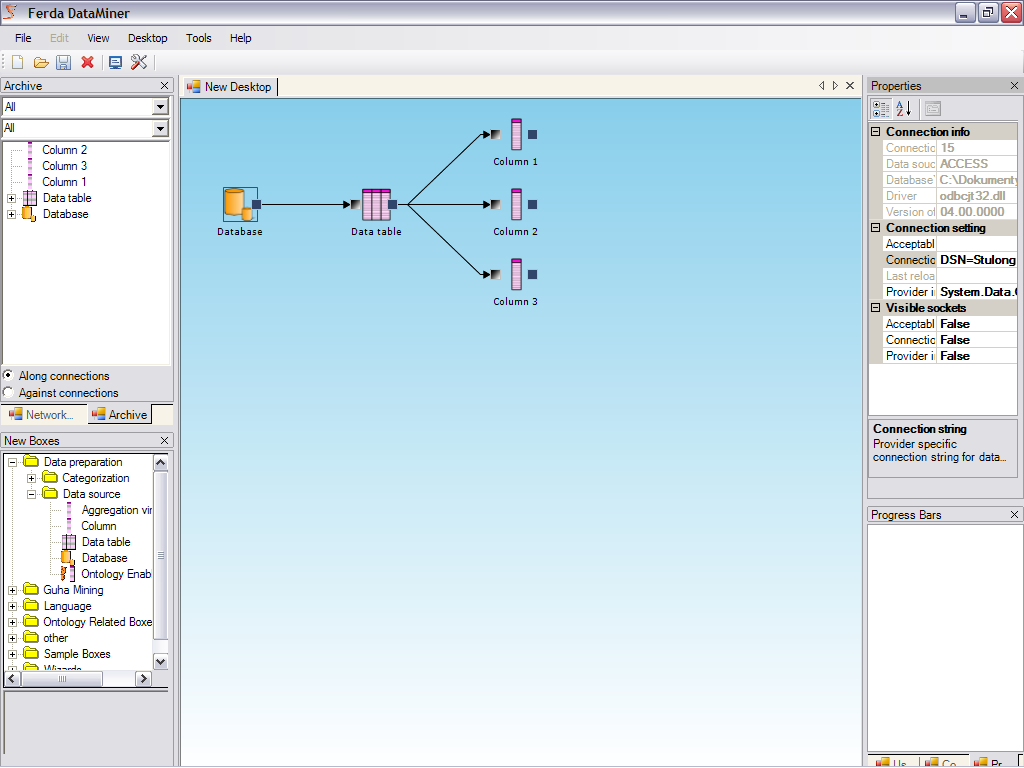
\includegraphics{Ferda.png}}}
\caption{The Ferda environment}
\label{fig:Ferda}
\end{figure}

Besides the desktop, the integrated environment shown on Figure~\ref{fig:Ferda} also features other components.
Among other, \emph{properties of boxes} are shown in the standard property grid component (upper-left component of the interface). 
The user may even create several desktops, and all the boxes that have been created are accessible via the \emph{archive of boxes} (upper-right component). 
A detailed description of all the components can be found in \cite{Ferda} or in project documentation.

\subsection{Modularity} \label{Modularity}
Ferda was designed according to the principles of modularity. 
The program runs on the \emph{Ice middleware layer}\footnote{\url{http://www.zeroc.com}}, which supports multiplatform communication of Ferda modules over the network. 
\emph{Box} is, obviously, the most important type of module in Ferda. 
The user can write boxes in different programming languages and easily add them to the system. 

As stated before, we designed the notion of box so as to represent a function rather than a phase of the data mining process. 
This allows for powerful tuning of the functionality of boxes. 
By implementing programming constructs such as the \emph{lambda} box or the \emph{if-then-else} box, the user can take advantage of a recursive programming language and create their own programs by connecting boxes. 
\cite{Kovac} provides more details. 
%
\emph{Setting module} is another type of Ferda module used in this work, which can be used to retrieve the value of a socket. 
For example, we use a setting module to retrieve the connection string to access a database. 
The connection string is a string property, but it is hard for a non-expert user to write this string correctly. 
Therefore a dialog is shown that helps the user with creation of the connection string.  

\subsection{GUHA Compliance}
Ferda complies with the GUHA method principles. 
The system implements 6 non-relational GUHA procedures with the ability to construct so called \emph{Boolean attributes} \cite{Disjunctions}. 
The system also implements two multi-relational GUHA procedures \cite{Kuzmin} and an algorithm for construction of GUHA decision trees \cite{ETree}. 